\section{Ontologies}

\begin{frame}{\insertsection}
    \blockquote[{{\cite[p. 290]{russell2022ArtificialIntelligenceModern}}}]{The word ontology means a particular theory of the nature of being or existence. The ontology determines what kinds of things exist, but does not determine their specific properties and interrelationships.}
    
    \medskip
    
    An ontology is a vocabulary of a chosen domain.

    \medskip

    An ontology is a \blockquote[\cite{guarino2009WhatOntology,borst1997ConstructionEngineeringOntologies}]{formal specification of a shared conceptualisation}.

    \medskip

    An ontology is a knowledge model.
    
\end{frame}

\begin{frame}{\insertsection}
    An ontology is often described as a set of \alert{triples}:

    $$(\quad\text{subject}\quad,\quad\text{predicate}\quad,\quad\text{object}\quad)$$

    where:
    \begin{itemize}
        \item subject and object are usually \alert{concepts}, their individuals, or literals,
        
        \item predicate is an object or a data \alert{property}.
    \end{itemize}

    \medskip
    An example:

    $$(\quad\text{a dog}\quad,\quad\text{can play with}\quad,\quad\text{a ball}\quad)$$
\end{frame}

\begin{frame}{\insertsection}
    Common concepts related to the domain of ontologies:

    \begin{description}
        \item [\Ac{RDF}] is a standard for representing data on the web using triples. It helps link and describe information so computers can understand relationships between different concepts.

        \item [\Ac{OWL}] is a language for creating complex models of knowledge (i.e. ontologies) by defining relationships, classes, and rules. It extends RDF to enable reasoning, such as inferring new facts from given data.
    \end{description}
\end{frame}

\begin{frame}{\insertsection}
    \customFigure[0.9]{% how wide is the figure?
        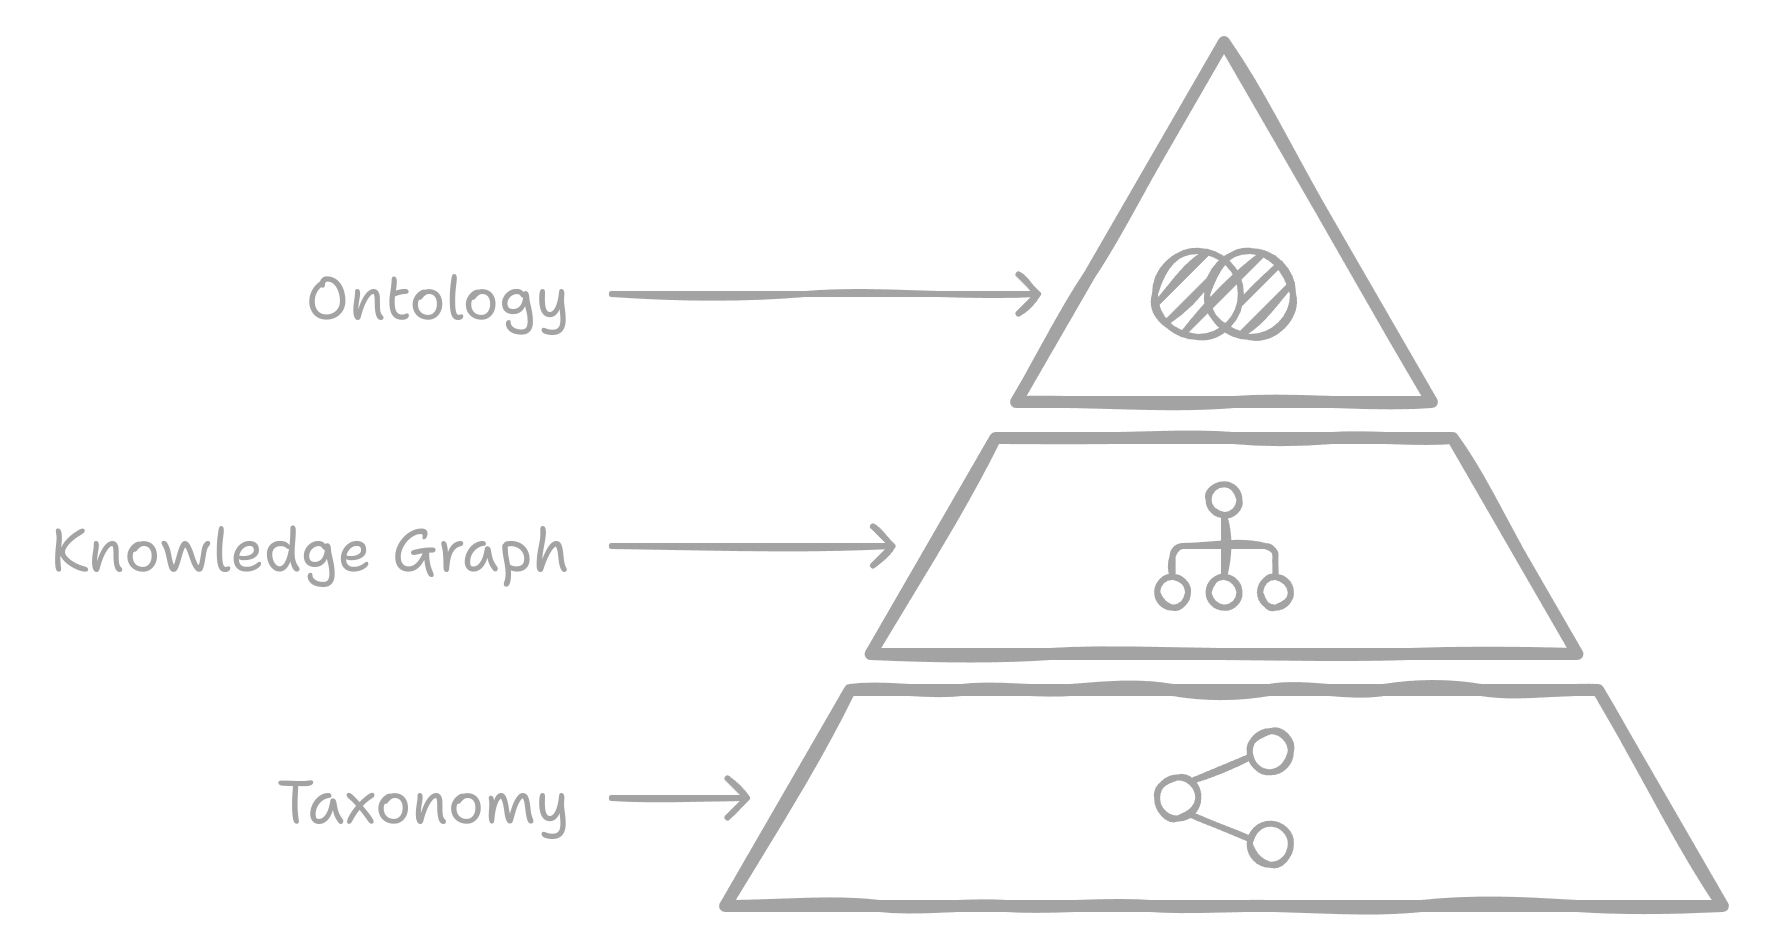
\includegraphics{Documents/241119 DSC Europe/Figures/taxonomy knowledge graph ontology.png}
    }{Hierarchical visualisation of information structures taxonomy, knowledge graph, and ontology}{taxonomy knowledge graph ontology}
\end{frame}

\begin{frame}{\insertsection}
    \customFigure[0.9]{% how wide is the figure?
        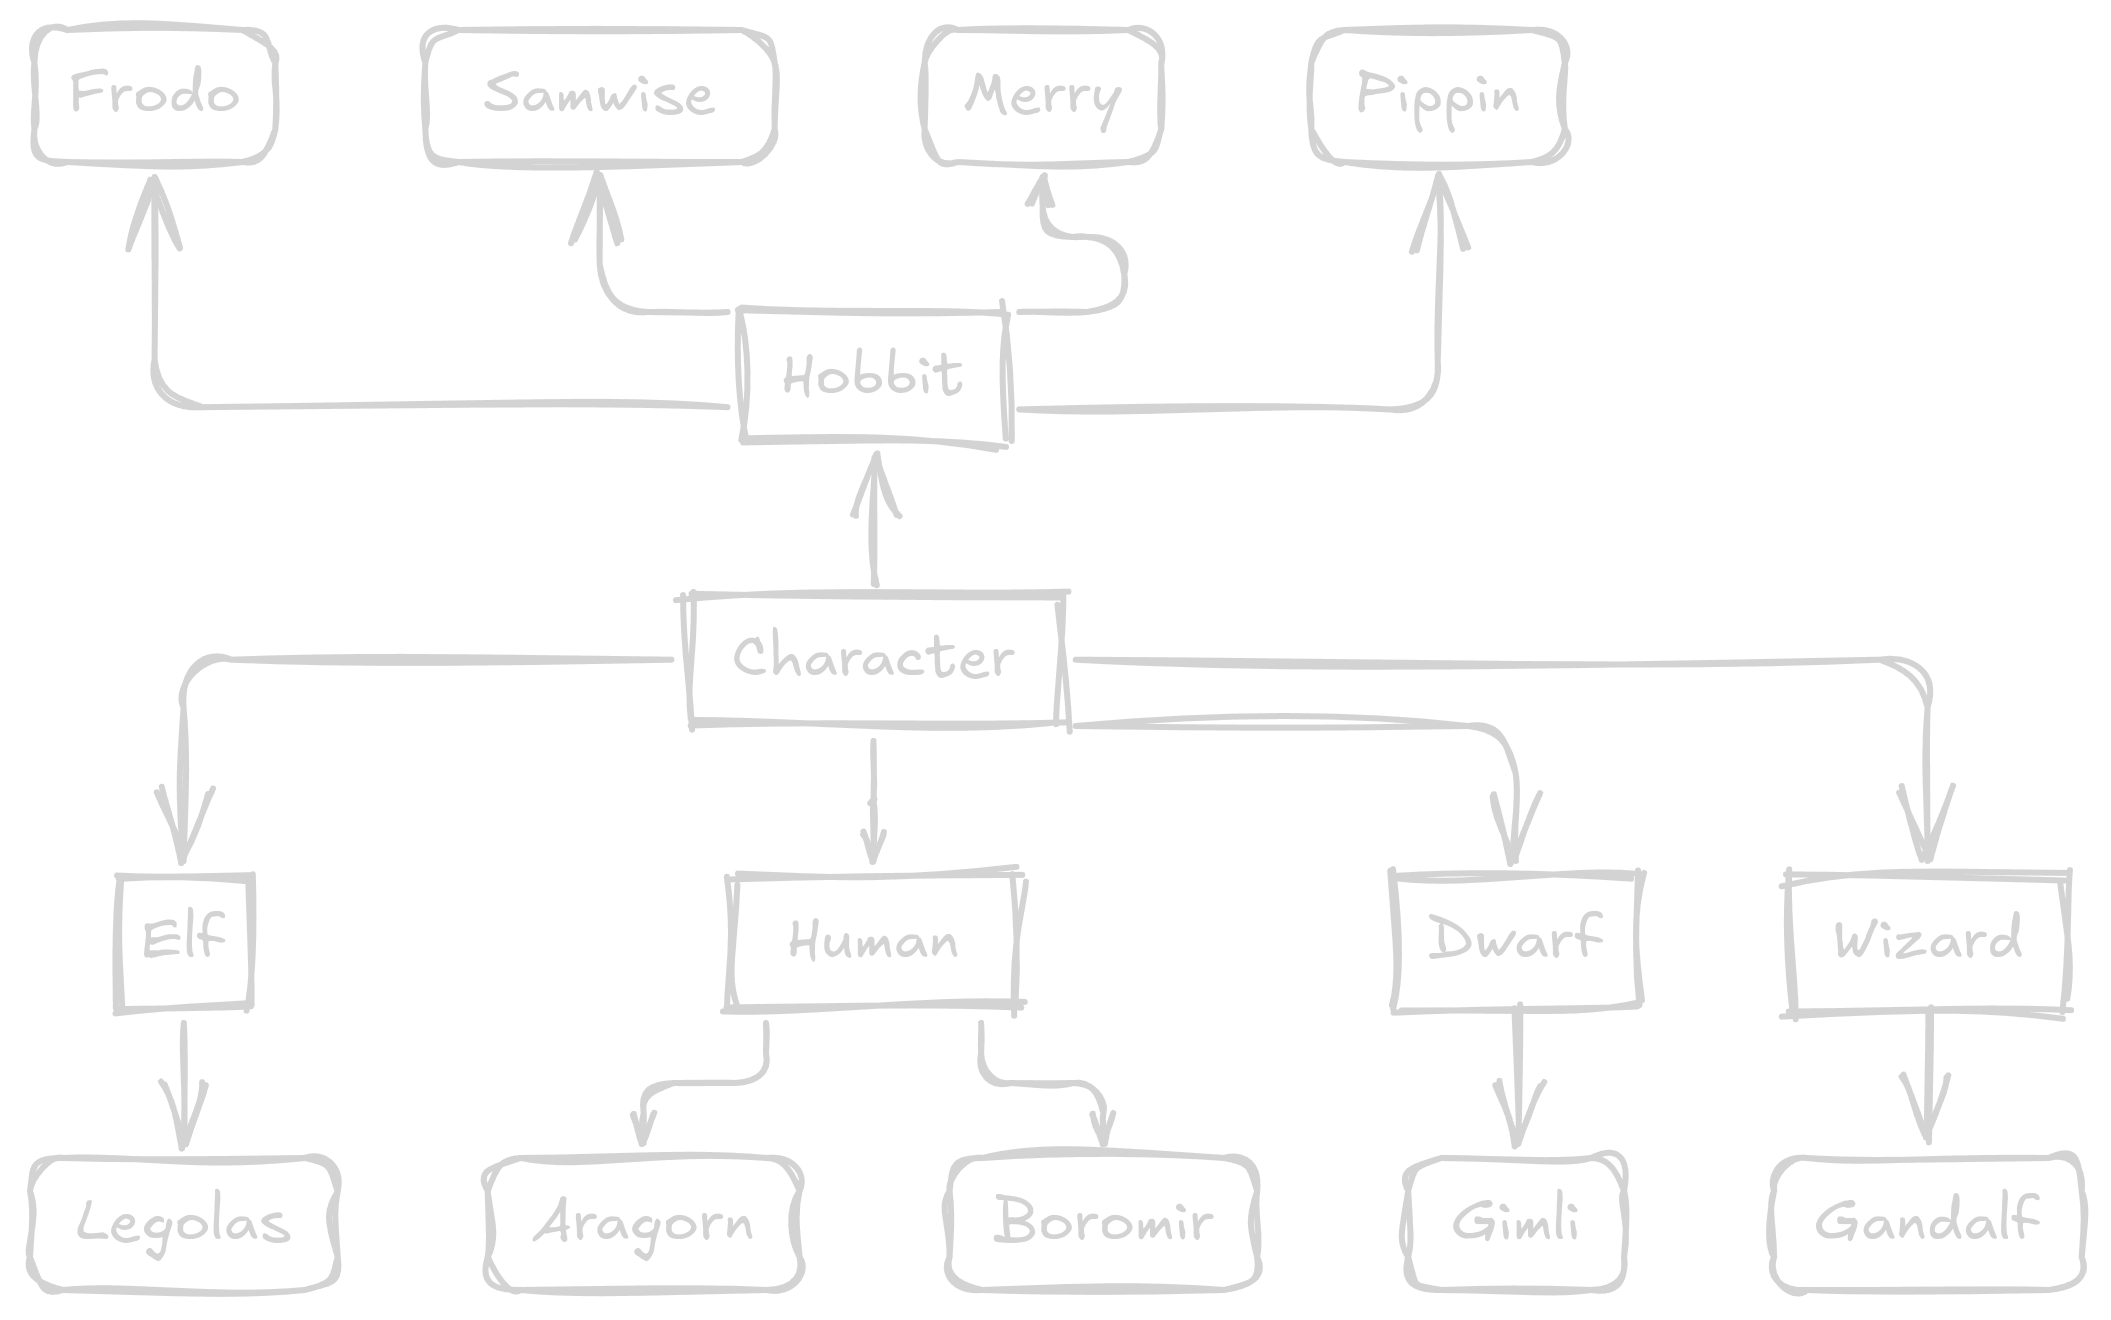
\includegraphics{Documents/241119 DSC Europe/Figures/Taxonomy the Lord of the Rings characters.png}
    }{Taxonomy of the selected concepts of the Lord of the Rings novel by J.~R.~R.~Tolkien \cite{tolkien2007LordRings}}{taxonomy lotr}
\end{frame}

\begin{frame}{\insertsection}
    \customFigure[0.7]{% how wide is the figure?
        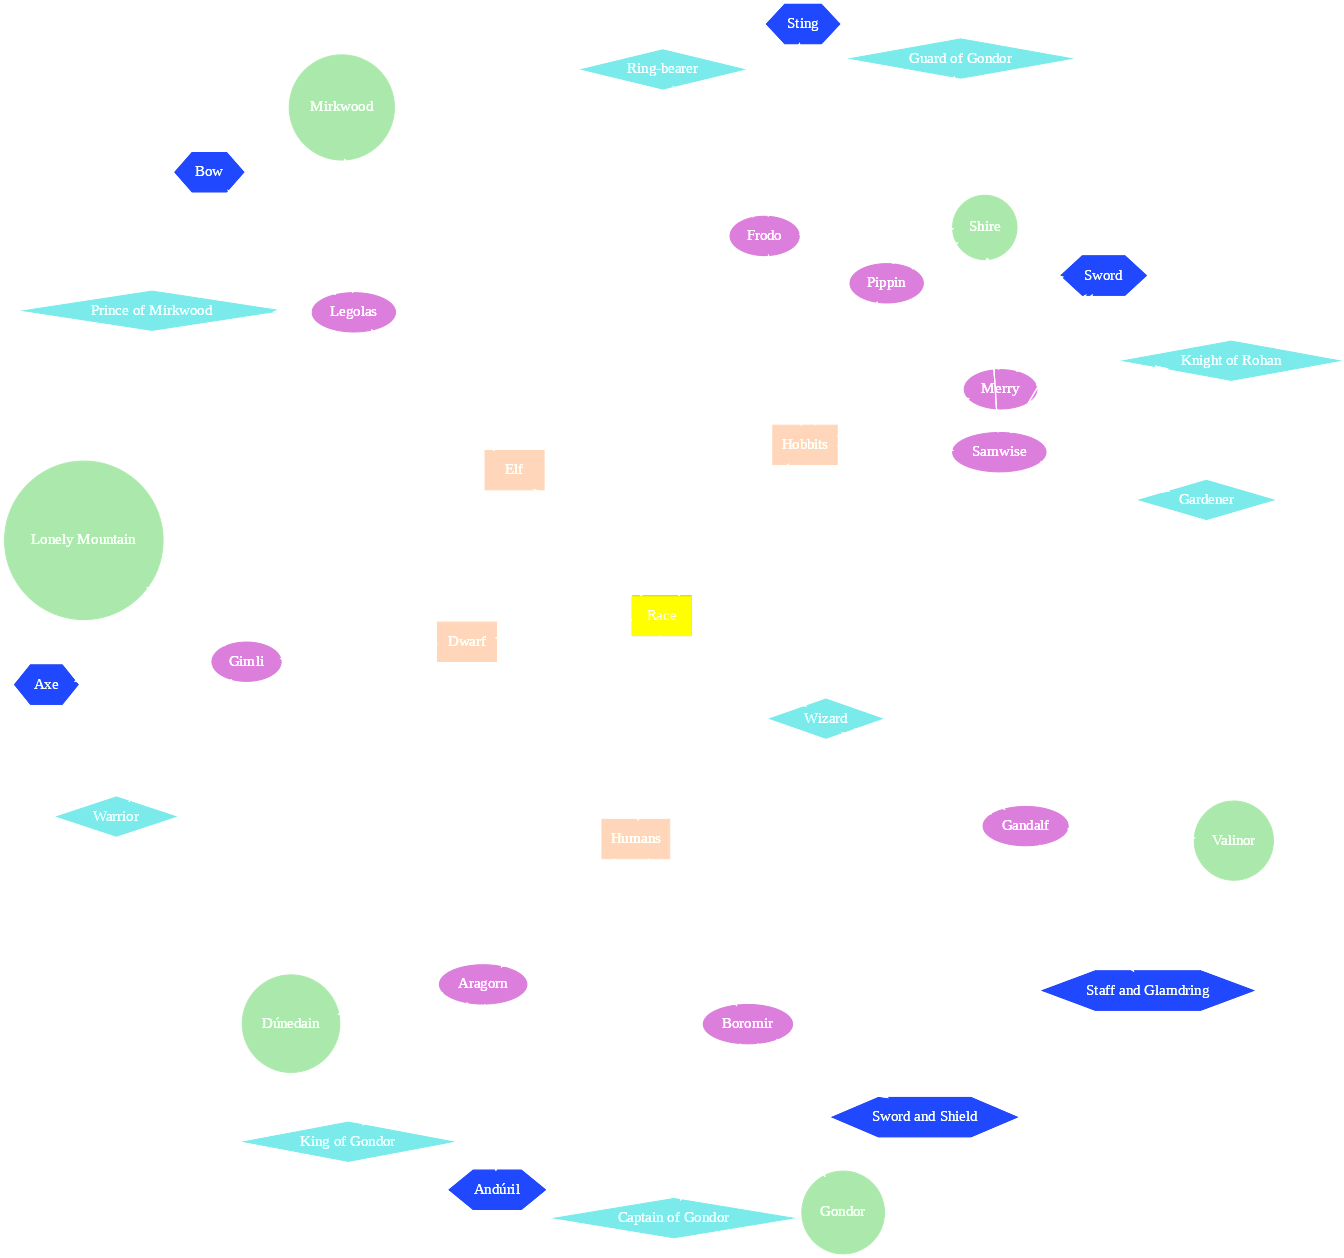
\includegraphics{Documents/241119 DSC Europe/Figures/Knowledge graph Lord of the Rings dark.png}
    }{Knowledge graph of the selected concepts of the Lord of the Rings novel by J.~R.~R.~Tolkien}{knowledge graph lotr}
\end{frame}


\begin{frame}{\insertsection}
    \customFigure[0.9]{% how wide is the figure?
        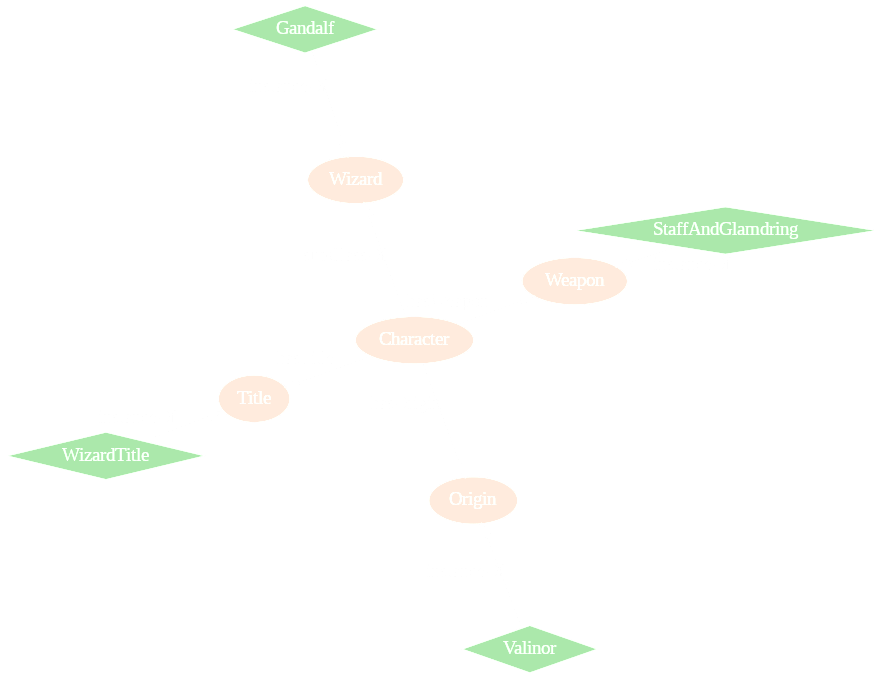
\includegraphics{Documents/241119 DSC Europe/Figures/Ontology exmaple visualisation Lord of the Rings dark.png}
    }{Ontology visualisation of the selected concepts of the Lord of the Rings novel by J.~R.~R.~Tolkien}{ontology lotr}
\end{frame}

\begin{frame}[fragile]{\insertsection}

    An ontology is more than a set of related concepts.

    \begingroup
    \setlength{\columnsep}{3em}
    \begin{multicols}{3}
        \begin{listing}
        \mintedFileText[firstline=7, lastline=18]{Documents/241119 DSC Europe/Figures/ontology example.txt}
        \end{listing}
        
        \begin{listing}
        \mintedFileText[firstline=20,lastline=31]{Documents/241119 DSC Europe/Figures/ontology example.txt}
        \end{listing}
        
        \begin{listing}
        \mintedFileText[firstline=33,lastline=46]{Documents/241119 DSC Europe/Figures/ontology example.txt}
        \end{listing}
    \end{multicols}
    \endgroup
\end{frame}

\begin{frame}[fragile]{\insertsection}
    An ontology is a \alert{shared} vocabulary of a chosen domain.

    \mintedFileText[firstline=8, lastline=8]{Documents/241119 DSC Europe/Figures/ontology example.txt}
\end{frame}

\begin{frame}[fragile]{\insertsection}
    \customFigure[1.3]{% how wide is the figure?
        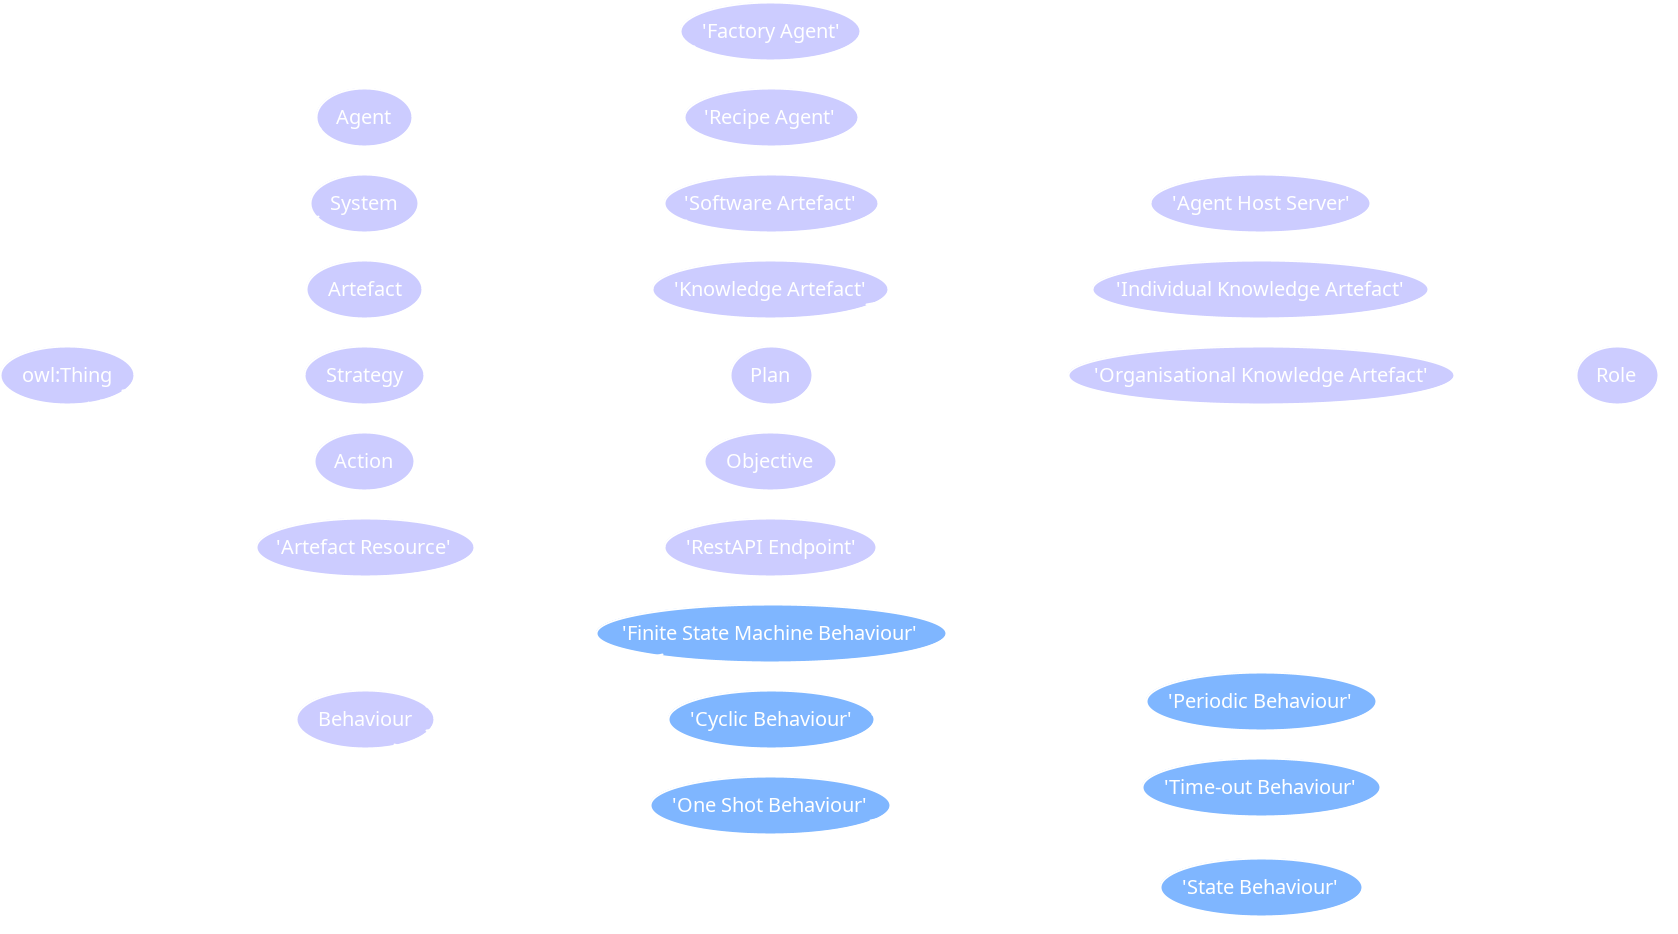
\includegraphics{Documents/241119 DSC Europe/Figures/onto dark.png}
    }{Concepts of the \magoag ontology}{knowledge graph lotr}
\end{frame}

\begin{frame}[fragile]{\insertsection}
    \begin{block}{RecipeWorld example}
        RecipeWorld \cite{Fontana2015recipeWorld} is an agent-based model comprising three distinct foundational elements: recipes, orders, and agents. In general, agents within recipeWorld can be considered as \alert{service providers} and \alert{service consumers}.

        \medskip
        \alert{Order} agents need services as detailed in their recipes, while \alert{factory} agents provide a subset of all the services available in the system.

        \medskip
        The original framework's goal is to simulate \blockquote[\cite{Fontana2015recipeWorld}]{the emergence of networks out of a decentralized autonomous interaction.}
    \end{block}
\end{frame}

\activityFrame{Prot\'{e}g\'{e}}

\begin{frame}{\insertsection}
    There are several ways to work with ontologies using programming languages. 
    
    Let us take a look at \mintedInline{owlready2} for Python.
\end{frame}

\activityFrame{\mintedInline{owlready2}}
